\documentclass[17pt]{beamer}
\usepackage{graphicx}
\usepackage{tikz}
\usepackage{tikz-cd}
\usepackage{amsfonts}
\usepackage{amssymb}
\usepackage{amsmath}
\usepackage{amscd}
\usepackage{amsthm}
\usepackage{bbm}
\usepackage{fourier}
\usepackage[utf8]{inputenc}
\title{Semantics \\ and the \\ god's eye view}
\author{Hans Halvorson}
\date{June 7, 2018}
\setbeamertemplate{navigation symbols}{}%remove navigation symbols
\usepackage{eucal}
\setbeamercolor{normal text}{fg=black,bg=white}
\setbeamercolor{alerted text}{fg=red}
\setbeamercolor{example text}{fg=black}
\usepackage[absolute,overlay]{textpos}
\begin{document}
\def\2{\mathcal}
\def\7{\mathfrak}

\begin{frame}

\maketitle  %% the invariant content of equivalent theories

\end{frame}

\begin{frame}{\small introduction}

  \begin{description}
    \item[Ongoing series] Unintended consequences of the semantic view of
      scientific theories
    \item [Today's episode] How we were tricked into thinking that
      semantics moves us closer to the \textbf{god's eye
        view} \end{description}


\end{frame}


\begin{frame}{\small what is this god's eye view?}

\begin{itemize}
\item The aspiration for scientific objectivity, transcending our
  parochial differences
\item Not the French way of seeing things, or the German way, or a
  man's way, or a woman's way, or \dots
\end{itemize}

\end{frame}



\begin{frame}{\small what is the god's eye view?}

\begin{itemize}  
\item Optimists: rationalists and metaphysical realists
  such as Leibniz and Hegel
\item Pessimists: conventionalists and voluntarists such as Poincar\'e
  and Carnap
\end{itemize}


\end{frame}

\begin{frame}{\small god's eye view in contemporary philosophy}

\begin{itemize}
\item w.r.t. quantum theory, the phrase ``completing the circle''
  expresses aspiration for a god's eye view
% an open circle has a place for an agent who chooses how to use the
% formalism
\item w.r.t. metaphysics, the phrase ``cutting nature at the joints''
  expresses aspiration for a god's eye view
\end{itemize}


\end{frame}




\begin{frame}{\small what's a theory?}

Syntactic view of theories: A theory $T$ is a deductively closed
sentence in some first-order signature $\Sigma$.

\bigskip

Complaint: The syntactic view makes theories \emph{language-dependent}


\end{frame}


\begin{frame}{\small is semantics divine?}

Semantic view of theories: A theory $T$ is a class of models.

\bigskip 

Claim (van Fraassen): The semantic view liberates theories from
language-dependence


\end{frame}

\begin{frame}[fragile]{\small is semantics divine?}

\begin{tikzcd}
    & & \mathcal{M} & & \\
    T_1 \arrow{urr}{} & T_2 \arrow{ur}{} & & T_3 \arrow{ul}{} & T_4 \arrow{ull}{}
 \end{tikzcd}

\end{frame}

\begin{frame}{\small is semantics divine?}

different $\Sigma$ $\Rightarrow$ different $\mathcal{M}$

\bigskip \bigskip Example: Groups can be formulated in signature
$\Sigma _1=\langle \circ ,^{-1},e\rangle$, or in signature
$\Sigma _2=\langle \bullet \rangle$.

\bigskip \bigskip

But then $\mathcal{M}_1\neq \mathcal{M}_2$. \end{frame}

\begin{frame}{}

\textbf{Upshot:} A class of models is no less language-dependent
than a syntactically specified theory.

\bigskip

\begin{quote}
  We are suspended in language. (Niels Bohr) \end{quote}



\end{frame}

\begin{frame}{\small is semantics divine?}

$M=\langle \{ a,b,\langle a,a\rangle \} ,\{ \langle a,a\rangle \}
\rangle$

\bigskip

$N=\langle \{ a,b,\langle a,b\rangle \} ,\{ \langle a,b\rangle \}
\rangle$




\end{frame}


\begin{frame}{\small is semantics divine?}

  Claim (Nerlich, Suppe, van Fraassen, Sider, etc.): the semantic view
  liberates us from the need for correspondence rules

\end{frame}

\begin{frame}[fragile]{\small Putnam's paradox}

If $T$ is consistent, then $T$ is true

\bigskip \begin{tikzcd}
  & T \arrow{dl}{} \arrow[dashed]{dr}{} & \\
M \arrow[dashed]{rr}{} & & W \end{tikzcd}
  
\end{frame}


\begin{frame}{\small David Lewis' response}


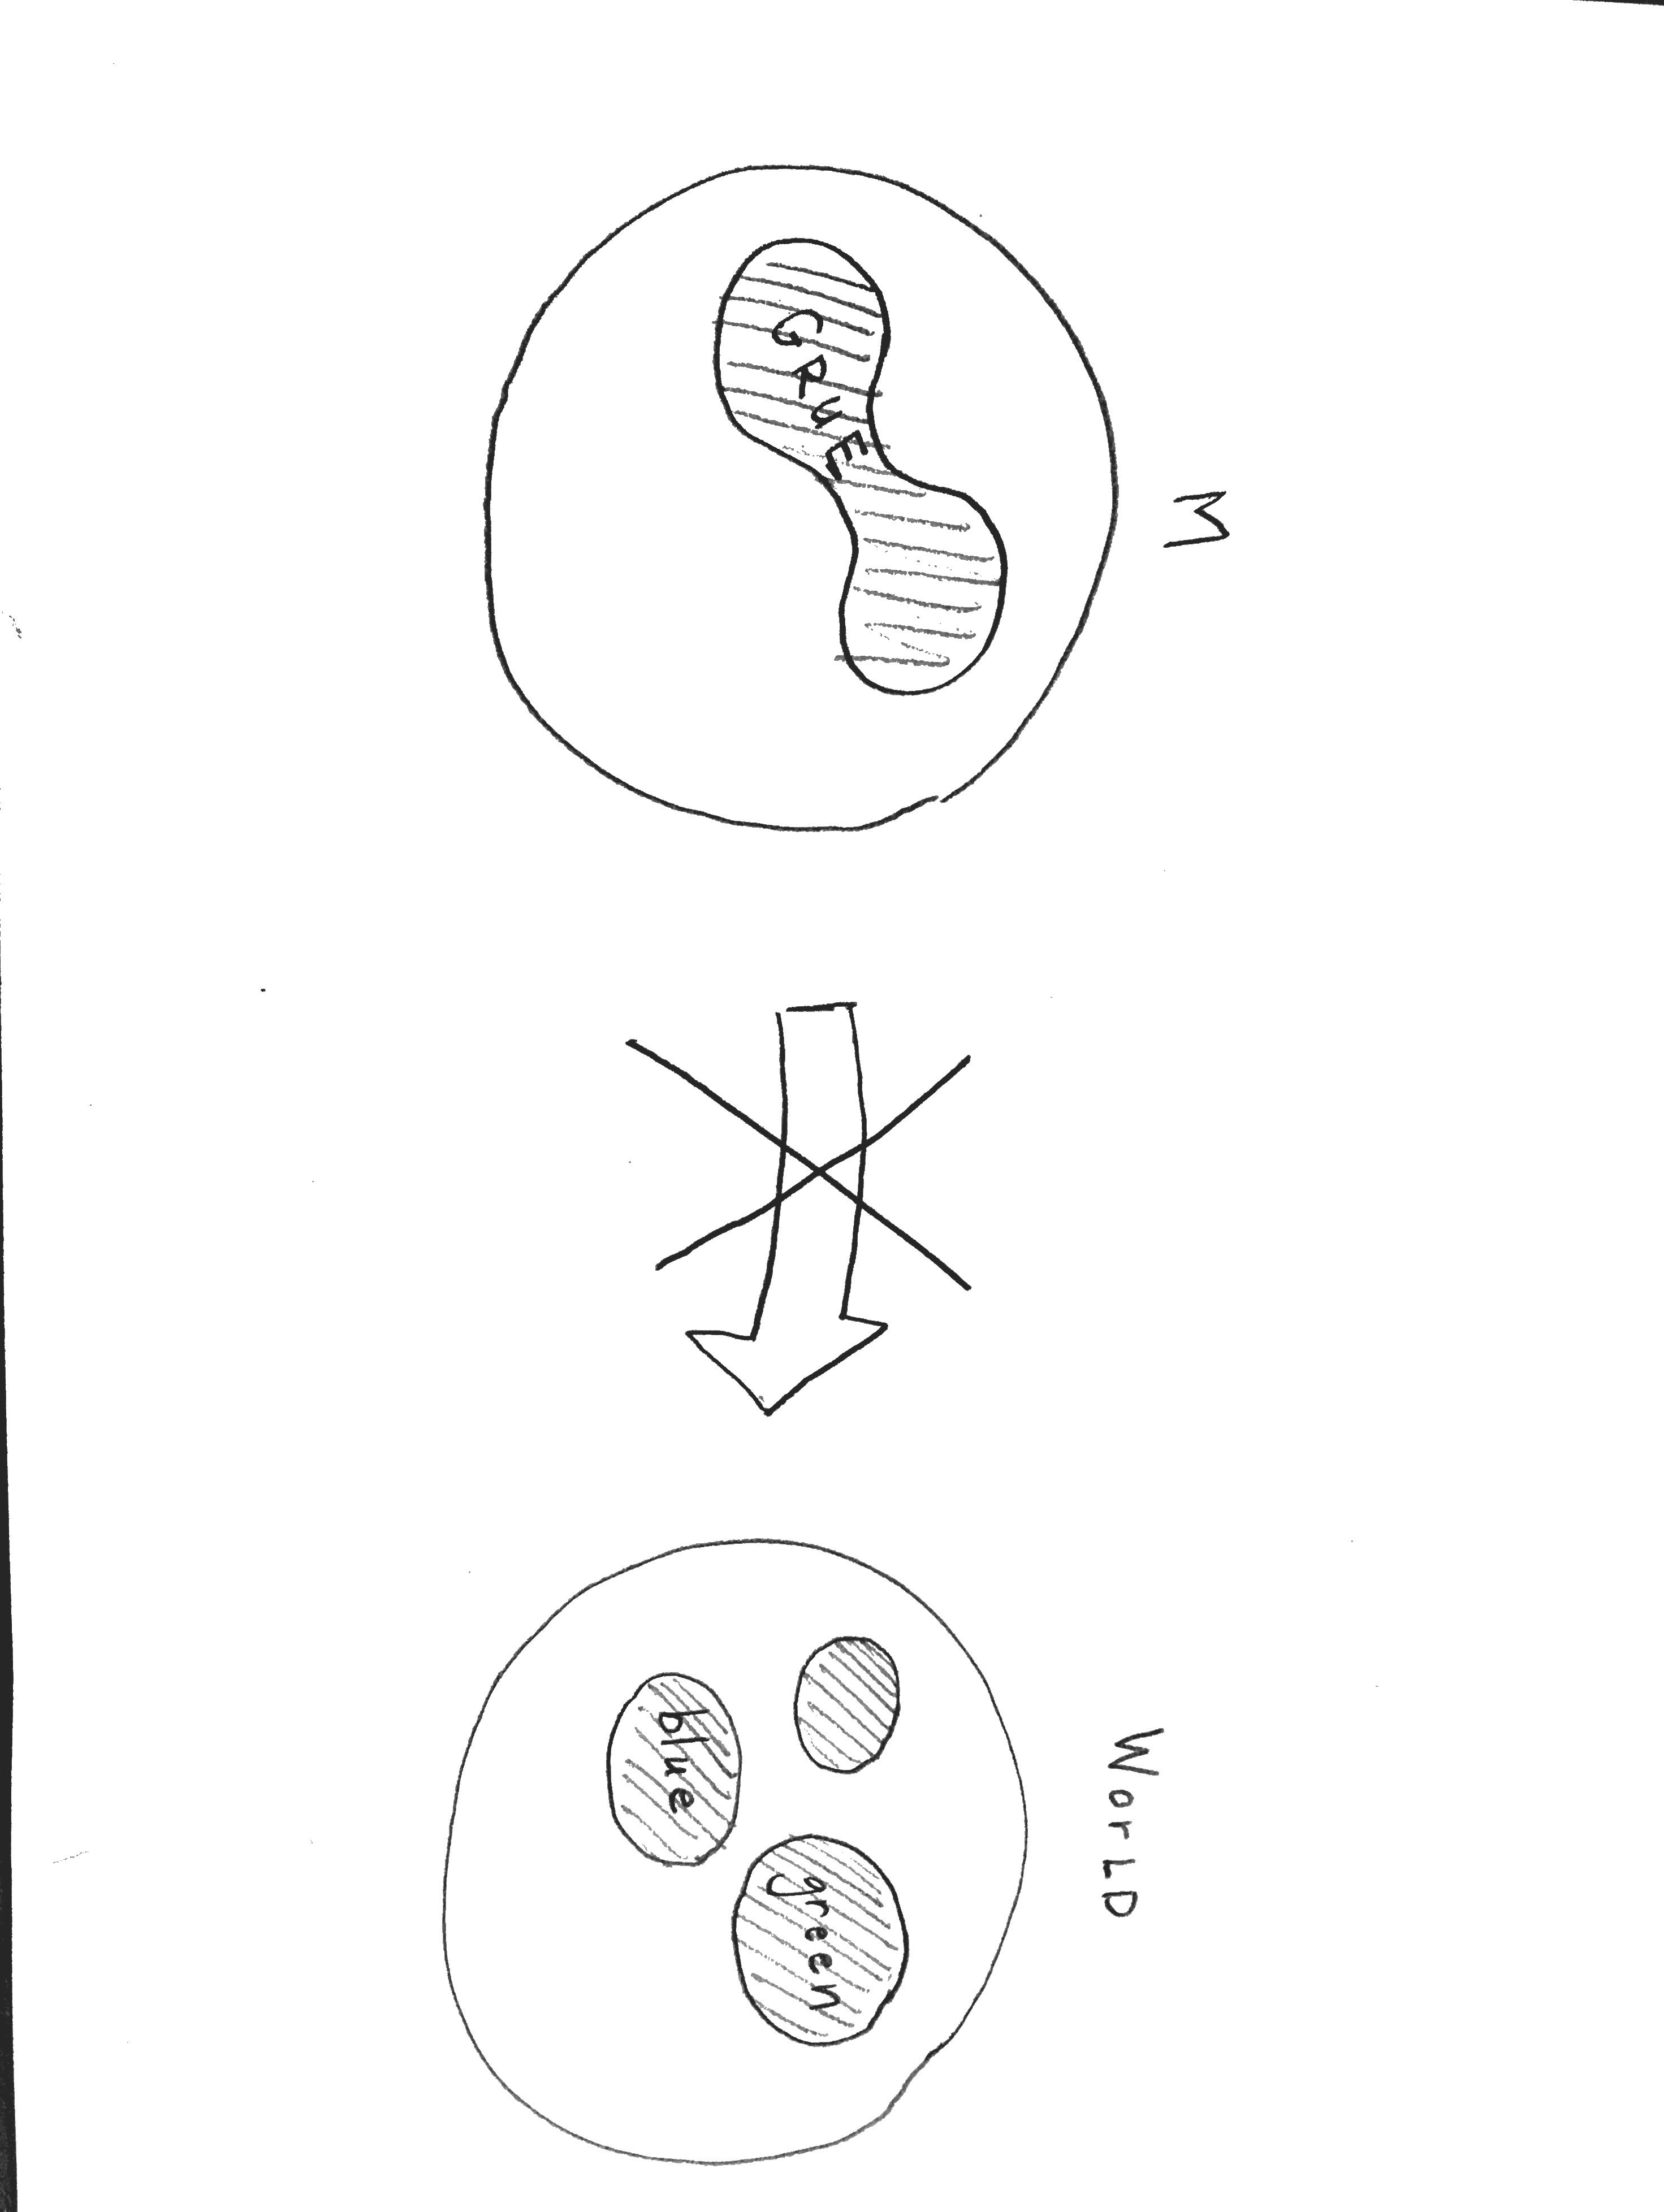
\includegraphics[angle=90,scale=0.08]{grue.jpg}

\end{frame}


\begin{frame}{\small who made Putnam God?}

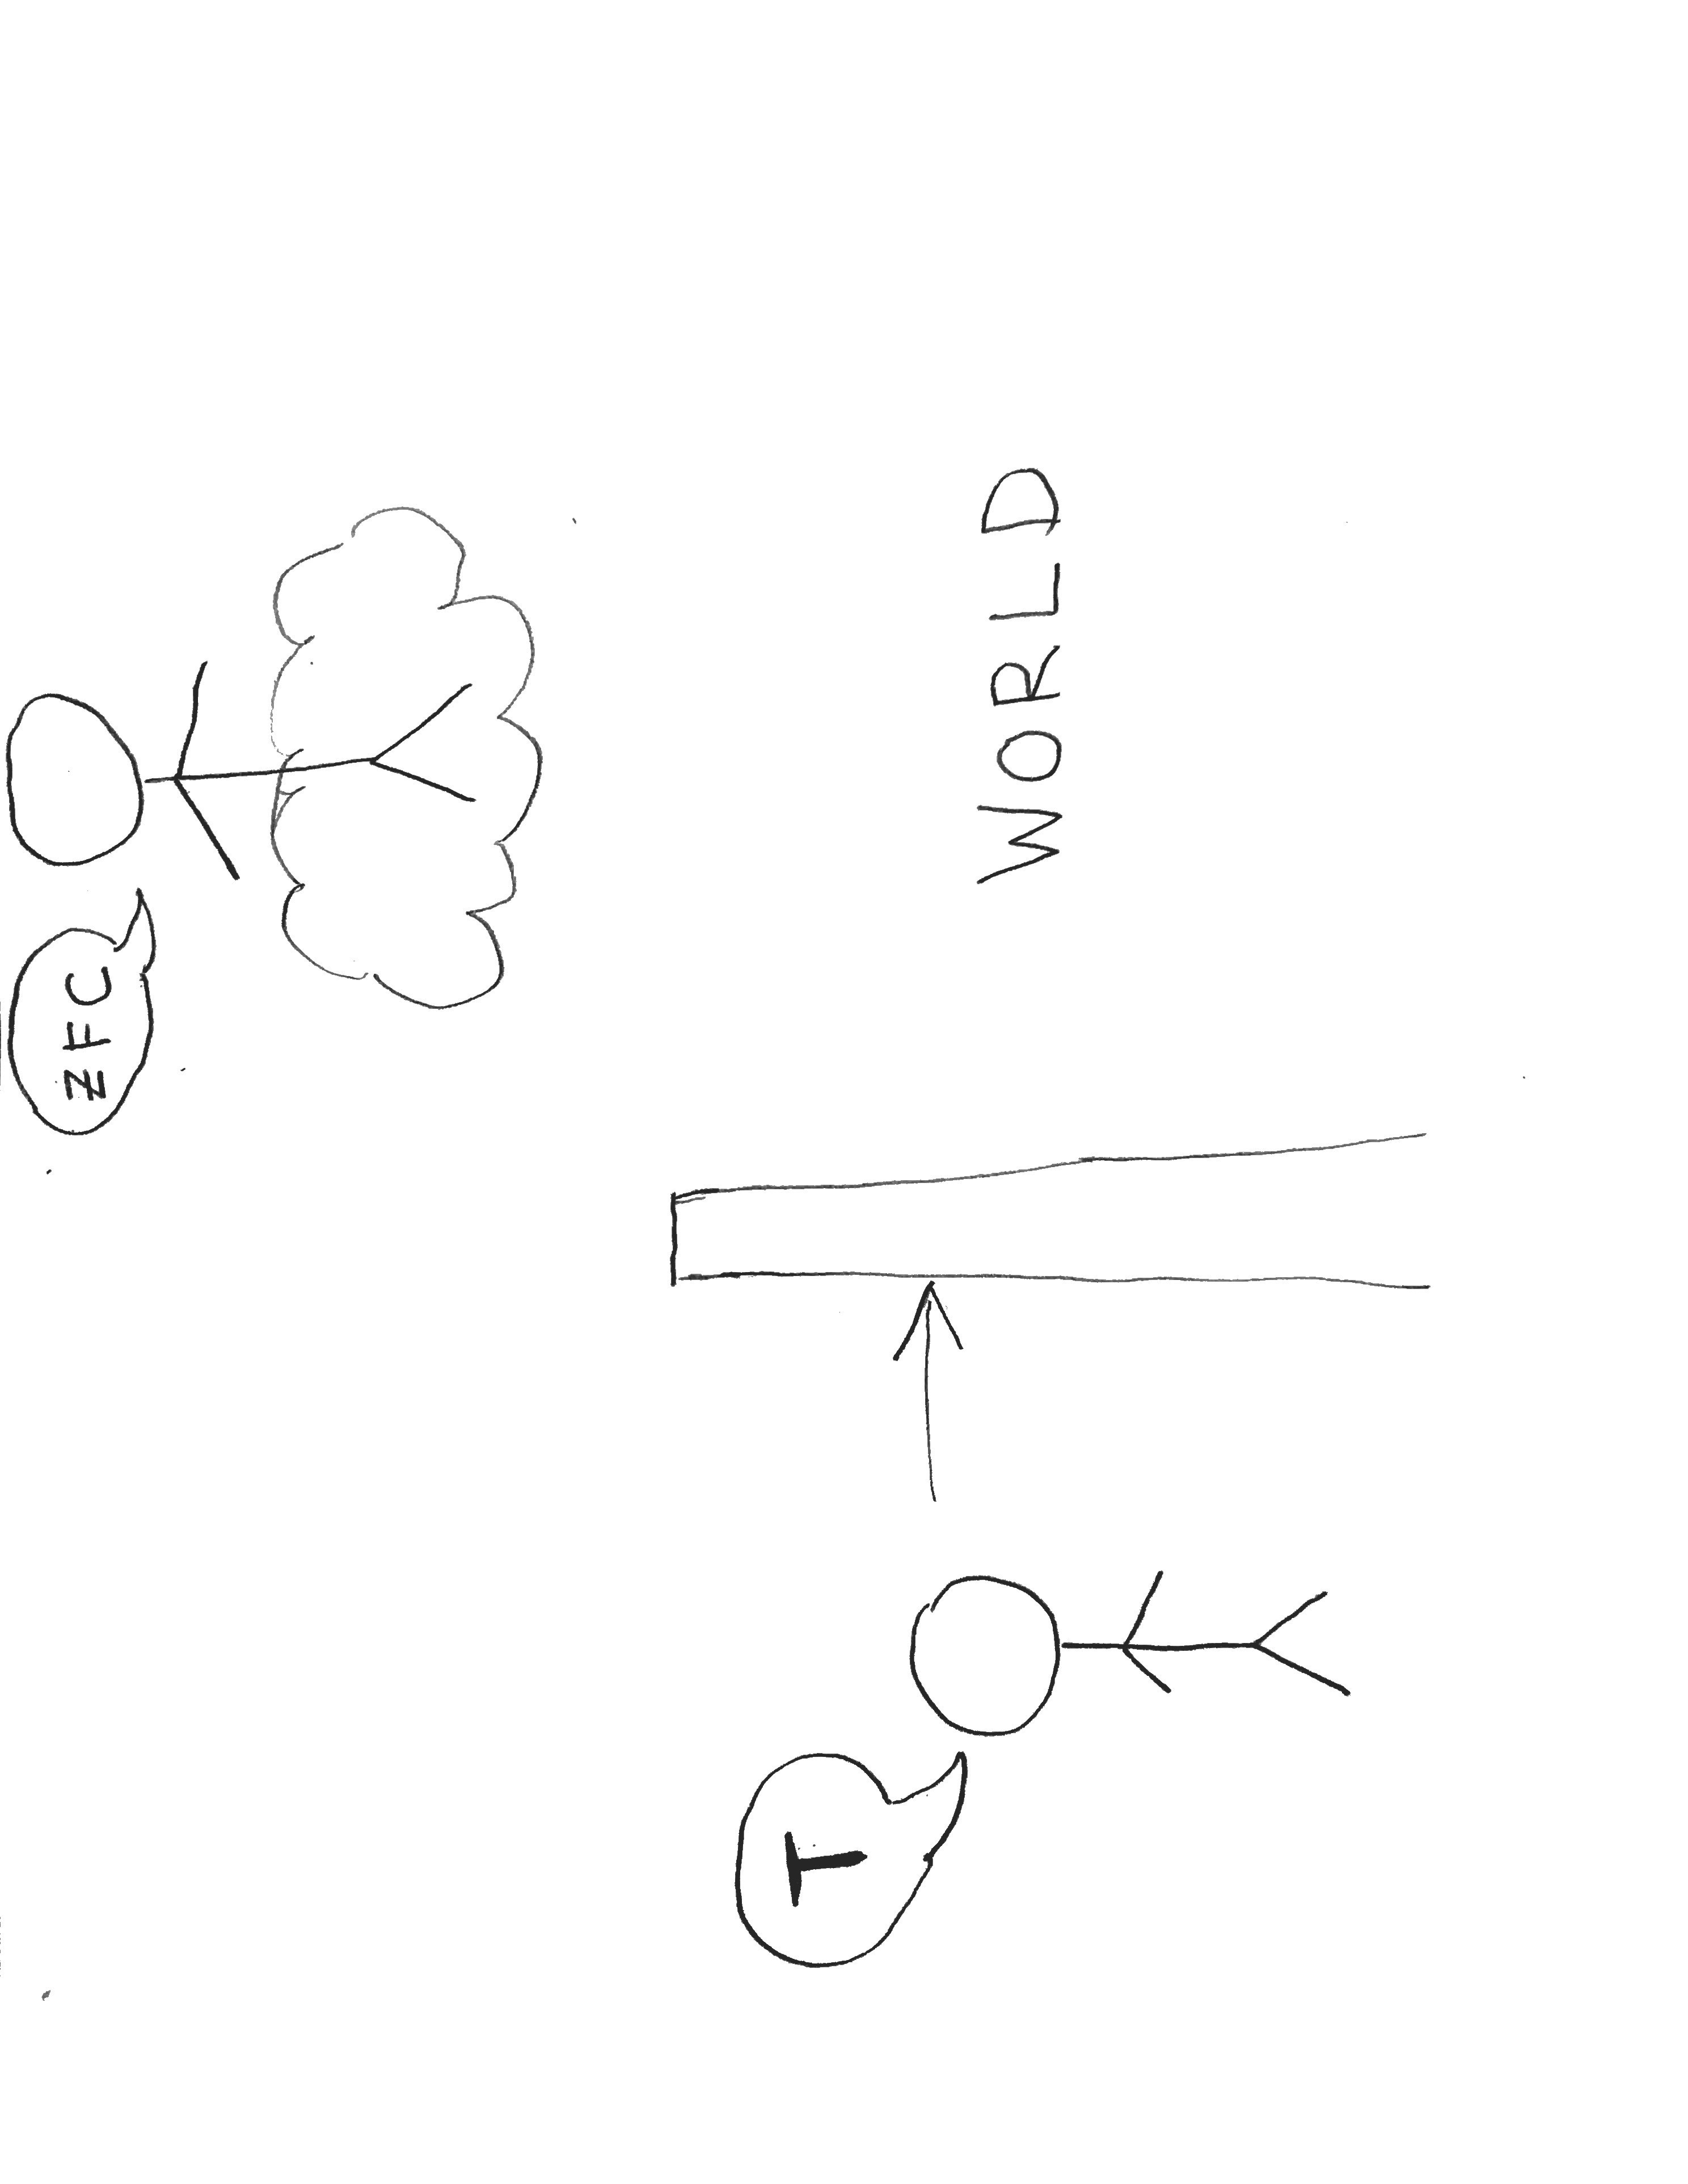
\includegraphics[scale=0.08,angle=-90]{gev.jpg}

\end{frame}

\begin{frame}{\small Putnam is people too}

  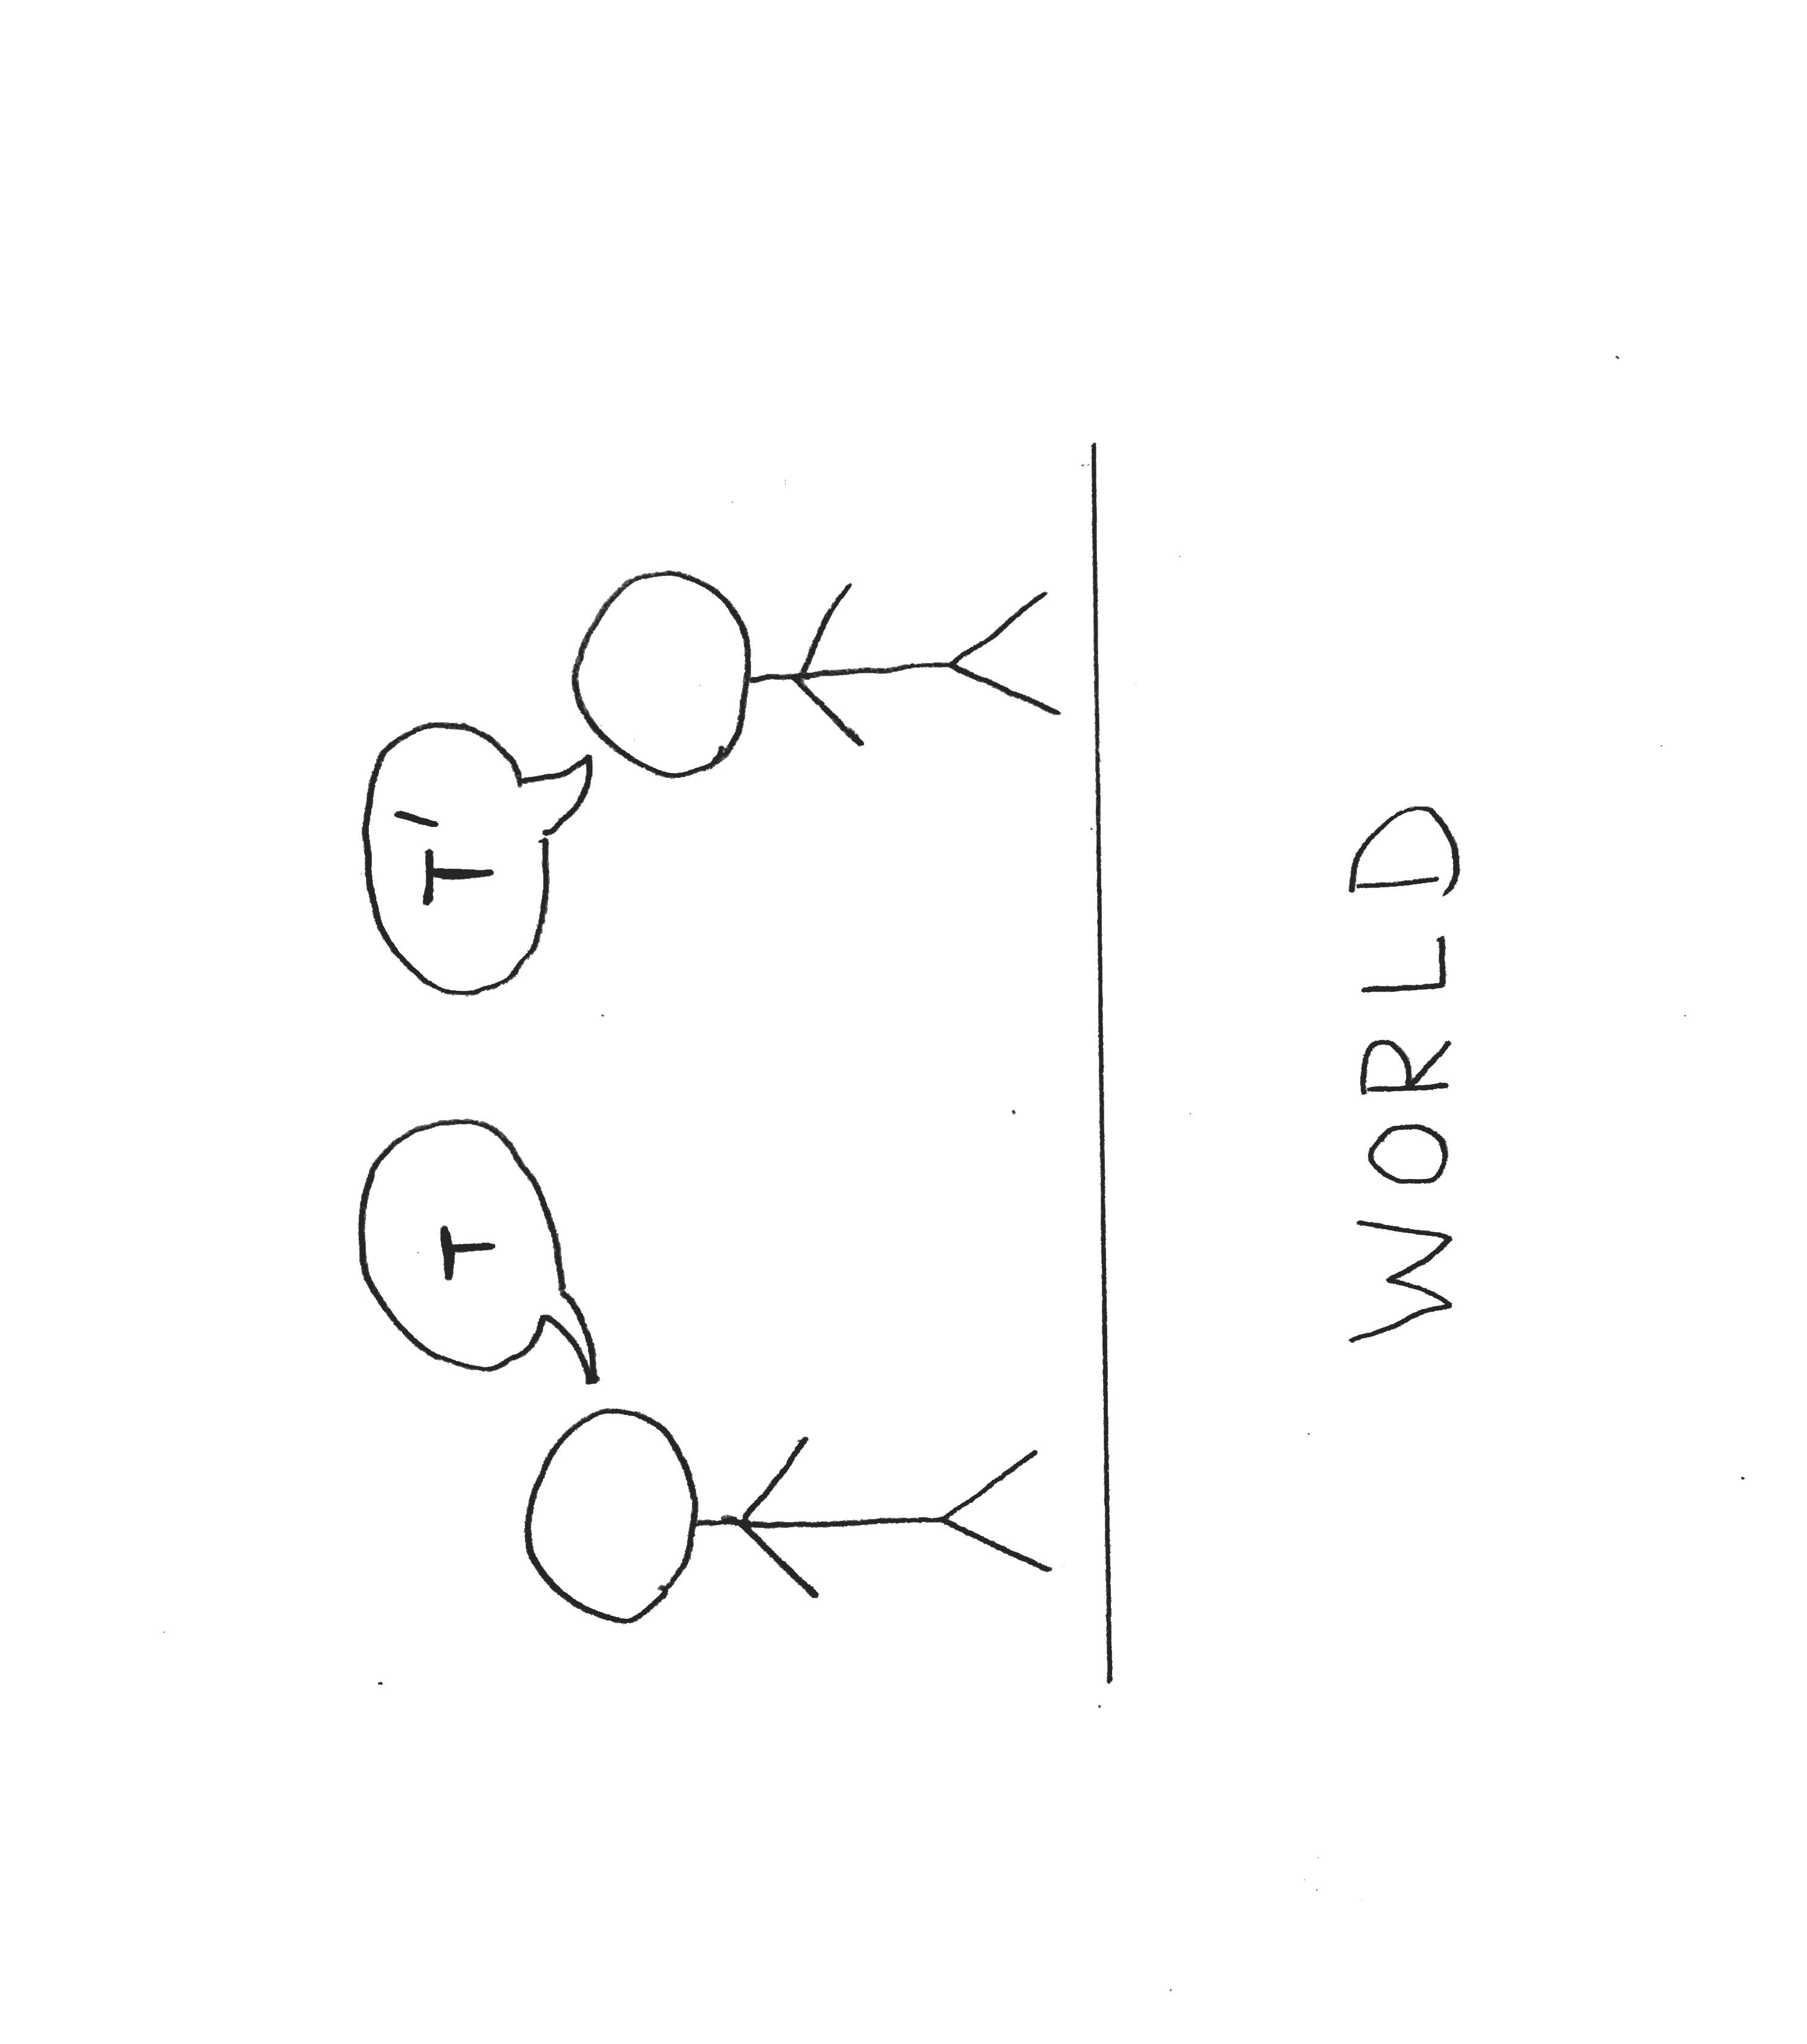
\includegraphics[scale=0.08,angle=-90]{peers.jpg}

\end{frame}

\begin{frame}{\small what Hilbert said to Frege}

  \begin{itemize}
    \item Hilbert: all consistency proofs are relative consistency proofs
    \item To say that a theory $T$ is consistent (in the precise
      technical sense) means that it has an interpretation into
      another theory ZFC
  \end{itemize}

\end{frame}


\begin{frame}{\small Cassirer against g-e-v}

Popular view: accepting GTR amounts to believing that the WORLD
is isomorphic to a Lorentzian manifold. 

\bigskip

Cassirer's view: accepting GTR is more akin to choosing a pair of
eyeglasses.

% It's not that we assert that two concrete (pre-existing)
% things are similar; rather, we build an abstract  mathematical
% artifact

% only one of the two things here is an "object", i.e. the world is an
% object.

\end{frame}


\begin{frame}{\small Kierkegaard against g-e-v}

  
  g-e-v excluded by the existence of \emph{genuine} theoretical
  choices, i.e.\ choices \emph{not} forced by Reason.  e.g. a choice
  of language, formalism, perspective, research topic, experiment,
  etc.


\end{frame}




\begin{frame}{\small Bohr against g-e-v}

  %% Favrholdt

  Describing the outcome of a measurement involves a genuine choice
  of how to apply the formalism

  

\end{frame}  





\end{document}



%%% Local Variables:
%%% mode: latex
%%% TeX-master: t
%%% End: